\section{Aufgabe I}

In diesem Versuch gilt für ein Skalenteil $1 Skt = 5,00 \cdot 10^{-5}\ \text{m}$.

Ausgewält wird das Öltröpfchen mit folgenden Messwerten:
Es gilt für doie Reaktionszeit $ \Delta t = 0,3\ \text{s}$ und für den Fehler der Skala gilt $\Delta s = 1\ Skt$
\begin{table}[h!]
    \centering
    \begin{tabular}{c c c}
        \hline
        Messung & Steigzeit $t_s$[s] & Fallzeit $t_f$[s]  \\
        \hline
        1 & $10,760$ & $18,590$ \\
        2 & $11,040$ & $20,560$ \\
        3 & $10,930$ & $21,860$ \\ 
        4 & $11,740$ & $18,270$ \\
        5 & $12,290$ & $20,650$ \\
        \hline
        & $\overline{t_s} = \SI{11,4 \pm 0,6}{\second}$ & $\overline{t_f} = \SI{20,0 \pm 0,8}{\second}$       
    \end{tabular}
\end{table}

Die Messtrecke beträgt hier immer $s =10 Skt$ also $s =5,00 \cdot 10^{-4}\ \text{m} = \SI{50}{\mm}$
Daraus ergibt sich mit:
\begin{equation}
    v = \frac{s}{t}
\end{equation}
Für die Geschwindigkeiten:
\[ \boxed{v_s = \SI{2,50 \pm 0,10}{\cdot 10^{-5}\ \tfrac{\meter}{\second}}}\]
\[ \boxed{v_f = \SI{4,41\pm 0,27}{\cdot 10^{-5}\ \tfrac{\meter}{\second}}}\]
Es gilt für den Fehler:
\begin{equation}
    \Delta v = \sqrt{(\frac{s}{t^2}\Delta t)^2 + (\frac{1}{t}\Delta s)^2}
\end{equation}

Daraus kann der Radius $r_0$ bestimmt werden nach Gleichung \ref{eq:r0} berechnet werden.
Mit:
\begin{itemize}
    \item $ g = \SI{9,81}{\tfrac{\meter}{\second^2}}$
    \item $\rho_{Öl} =  \SI{872,2}{\tfrac{\kg}{\meter^3}}$
    \item $\rho_{Luft} =  \SI{1,29}{\tfrac{\kg}{\meter^3}}$
    \item $\eta_0 = \SI{1,81}{\cdot 10 ^{-5}\ \tfrac{\N \second}{\meter^2}}$
\end{itemize}

\[r_0 = \SI{6,49 \pm 0,10}{\cdot 10^{-7}\ \meter} \]
Für den Fehelr gilt:
\begin{equation}
    \Delta r_0 = \sqrt{\frac{9 \eta_0}{2 (\rho_{Öl}- \rho_{Luft}) g}} \frac{1}{2 \sqrt{v_f}}\Delta v_f
\end{equation}

Zuerst wird der Korrekturfaktor $f(r_0)$ bestimmt durch Gleichung \ref{eq:f}:
\[f(r_0) = 0,8943 \pm 0,0012\]

Mit der Fehlerrechnung:

Daraus kann die Ladung $q$ des Tröpchens berechnet werden nach Gleichung \ref{eq:q}:

\[\boxed{q = \SI{1,56 \pm 0.12}{\cdot 10^{-19}\ \coulomb}}\]

Für den Fehler gilt:


\begin{align}
\Delta q^2 &= \left( \left(\frac{9\sqrt{2}\pi df \sqrt{\frac{\eta^{3}v_f}{g\rho}}}{U} + \frac{9\sqrt{2}\pi df \sqrt{\frac{\eta^{3}v_f}{g\rho}} (v_f+v_s)}{2U v_f}\right) \Delta v_f\right)^2 \notag\\ 
&\quad + \left(\frac{9\sqrt{2}\pi df \sqrt{\frac{\eta^{3}v_f}{g\rho}}}{U} \Delta v_s\right)^2 \notag\\
&\quad + \left(\frac{9\sqrt{2}\pi f \sqrt{\frac{\eta^{3}v_f}{g\rho}} (v_f+v_s)}{U} \Delta d\right)^2 \notag\\
&\quad + \left(\frac{-9\sqrt{2}\pi df \sqrt{\frac{\eta^{3}v_f}{g\rho}} (v_f+v_s)}{U^2} \Delta U\right)^2 \notag\\
&\quad + \left(\frac{9\sqrt{2}\pi d \sqrt{\frac{\eta^{3}v_f}{g\rho}} (v_f+v_s)}{U} \Delta f\right)^2
\end{align}

Der Der Mittelwert aus Excel für die 5 Ladungen ergibt:
\[\boxed{q = \SI{1,57 \pm0,05}{\cdot 10^{-19}\ \coulomb}}\]

Das entspricht einer Abweichung von $0,08\ \sigma$. Daher kann der Wert von Excel als genau betrachtet werden.
Durch die berücksichtigung von Fehlern und dem Runten von Zwischenergebnissen, entstehen leichte Abweichungen.
Diese sind aber nicht signifikant.

\newpage
\section{Aufgabe II}

\begin{figure}[h!]
    \begin{center}
        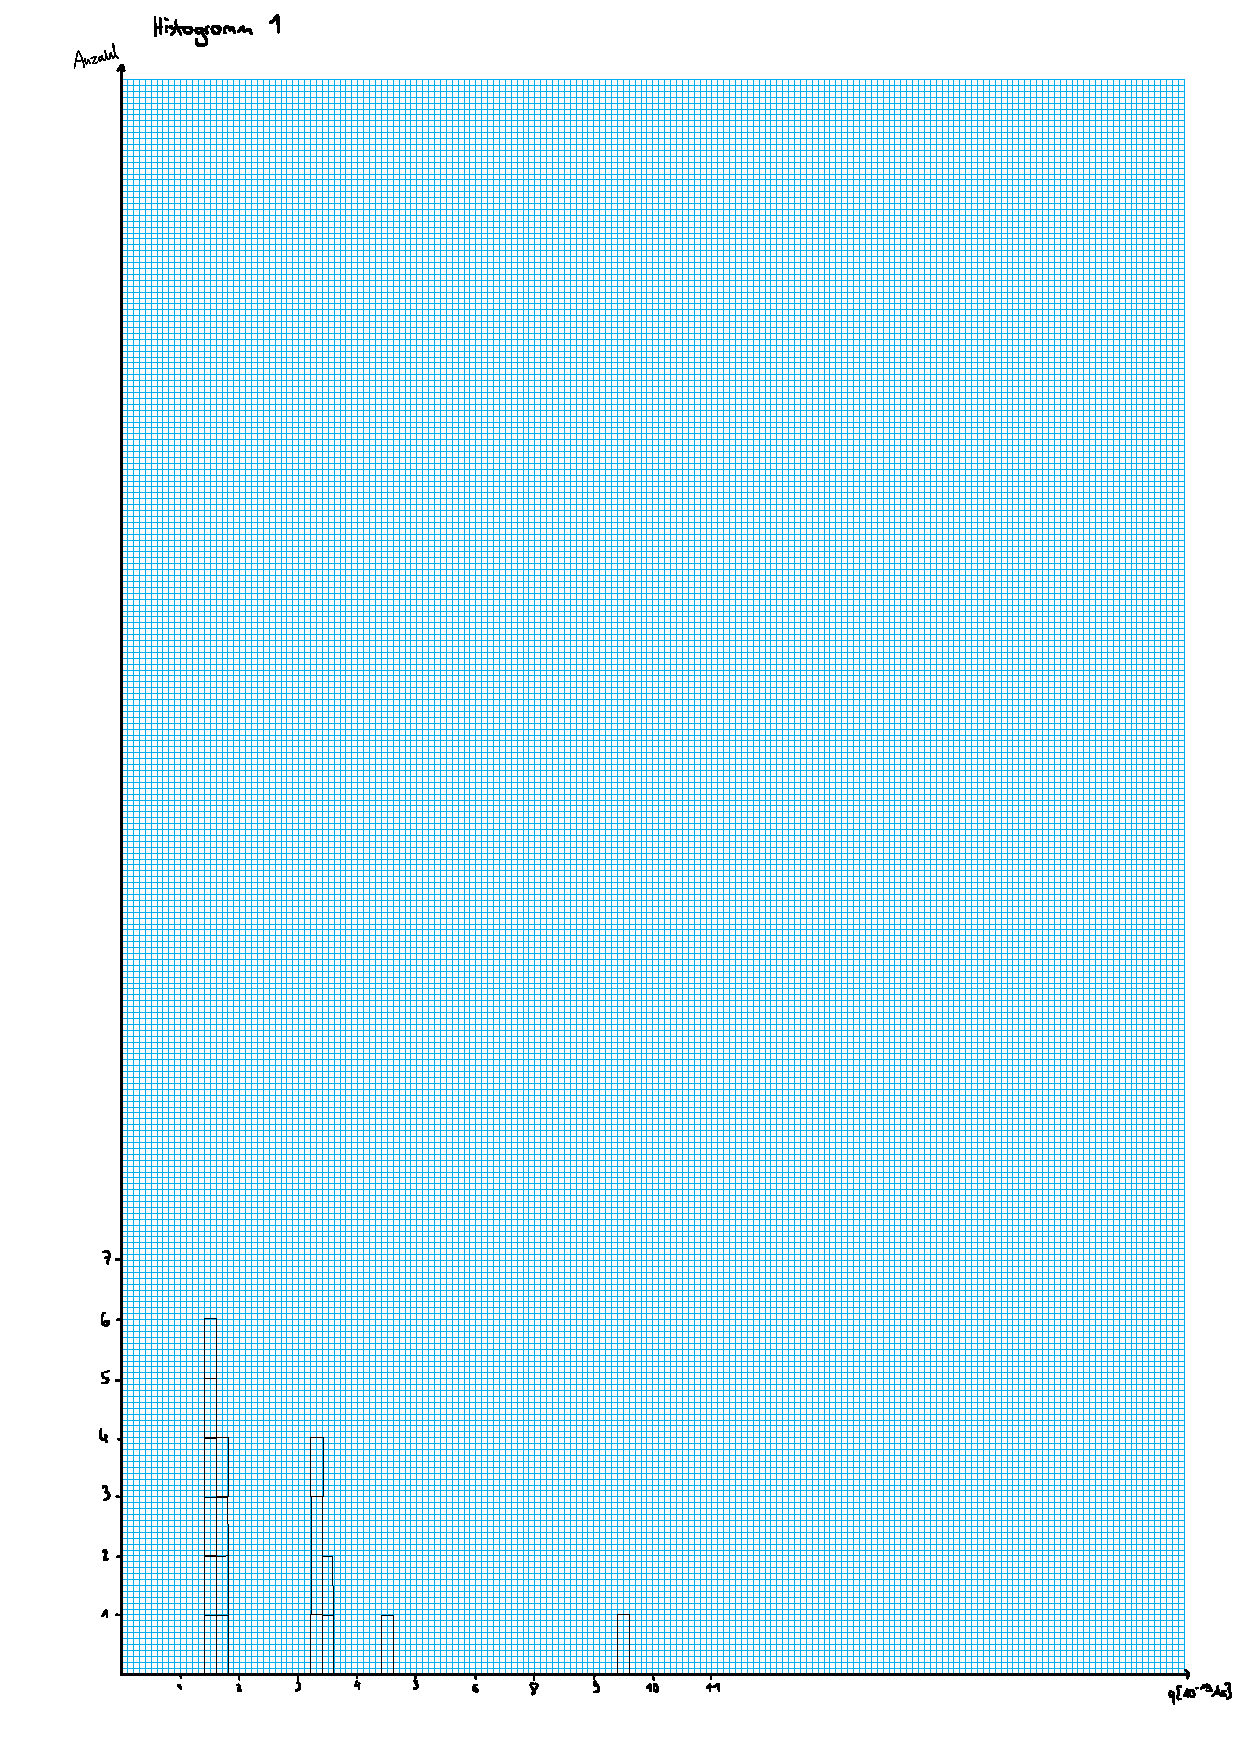
\includegraphics[width=.95\textwidth]{Histogramm22.pdf}
    \end{center}
\end{figure}

\newpage
\section{Aufgabe III}

Die Obergrenze für das Excel-Dokument wurde bei $2,4 \cdot 10^{-19}\ \text{C}$ gesetzt.
Ohne die Elementarladung zu kennen ist eine Abschätzung schwierig, da nicht ausgeschlossen werden kann,
dass nur gerade Anzahlen an Ladungen gemessen wurden. Da die Messung jedoch quantitativ ist,
kann ausgeschlossen werden, dass ausschließlich gerade Vielfache der Elementarladung gemessen wurden.
Da der Literaturwert bekannti ist, ist der Schwellenwert Sinnvoll. Dieser liegt genau zwischen $e$ und $2e$
es ist daher die einzige Grenze die gezogen werden kann, da die Werte einer Einzelladung gleichermaßen nach oben abweichen,
wie die von zwei nach unten.

\section{Aufgabe IV}
Der Fehler wird abgeschätzt mit folgender Formel:

\begin{equation}
    \frac{\Delta q}{q} = \sqrt{\left(\frac{3 \Delta s}{2s}\right)^2+\left(\frac{\Delta p}{2p}\right)^2+\left(\frac{3\Delta \eta}{2\eta}\right)^2+\left(\frac{\Delta d}{d}\right)^2+\left(\frac{\Delta U}{U}\right)^2}
\end{equation}

Die Vorfaktoren für $p$ und $\eta$ ergeben sich direkt als Faktor aus der Ableitung nach der jeweiligen Variable.

Bei $s$ ist das ganze nicht so offensichtlich. Zuerst müssen $v_f=\frac{s}{t_f}$ und $v_s=\frac{s}{t_s}$ so eingesetzt werden. Nun lässt sich das §
$s$ aus der Summe ausklammern und mit dem $s$-Faktor aus der Wurzel ergibt sich dann $\frac{3}{2}$ als Exponent für $s$. \\
Setzt man in diese Formel die gegebenen Werte ein erhält man:
Daraus ergibt sich mit dem Ablesefehler von 1 Skt der Relative Fehler von:

\[\boxed{\frac{\Delta q}{q} = 15\%}\]

\section{Aufgabe V}

\begin{table}[h!]
    \centering
    \begin{tabular}{c c c c c c c c c c c}
        \hline
        Messung &  $t_s$[s] &  $t_f$[s] & $v_s$[$10^{-5}$ m/s] & $v_f$[$10^{-5}$m/s] & $r_0$ [$10^{-7}$m] & $f$ & $q$[$10^{-19}$ C] \\
        \hline
        1 & $10,760$ & $18,590$ & $2,690 $ & $ 4,467$ & $6,656 $ & $ 0,897$ & $ 1,715$\\
        2 & $11,040$ & $20,560$ & $2,432 $ & $ 4,529$ & $6,571 $ & $ 0,895$ & $ 1,603$\\
        3 & $10,930$ & $21,860$ & $2,287 $ & $ 4,575$ & $6,604 $ & $ 0,896$ & $ 1,589$\\ 
        4 & $11,740$ & $18,270$ & $2,737 $ & $ 4,259$ & $6,372 $ & $ 0,893$ & $ 1,555$\\
        5 & $12,290$ & $20,650$ & $2,241 $ & $ 4,068$ & $6,228 $ & $ 0,890$ & $ 1,404$\\
        \hline
    \end{tabular}
\end{table}
Fehler der Einzelmessung:
\[ \sigma = 0,11 \]
Die Abweichung von Excel ergibt:
\[ \sigma_X = 0,097 \approx 0,10\]

Die Abweichungen stimmen in etwa überein. Die Differenz beträgt $0,01 $, weshalb das Ergebnis als in etwa übereinstimmend mit dem von Excel zu werten ist.
Das Excel Dokument berücksichtigt deutlich mehr Teilchen als diese Rechnung.

\section{Aufgabe VI}


\[\boxed{q = \SI{1,56 \pm 0.12}{\cdot 10^{-19}\ \coulomb}}\]

Verglichen mit dem Literaturwert $e =  1,602 176 634 \cdot 10^{-19} \text{C}$ ergibt sich eine abweichung von:
$0,35\ \sigma$.

Für den Wert, errechnet mit Excel ergibt sich:

\[\boxed{q_X = \SI{1,630 \pm 0.013}{\cdot 10^{-19}\ \coulomb}}\]

Also eine Abweichung von $2\ \sigma$ zum Literaturwert.
